%----------------------------------------------------------------------------
\chapter{\bevezetes}
%----------------------------------------------------------------------------

\section{Motivation}

The navigation of mobile robots has been a dynamic area of research, with significant advancements worldwide. For autonomous vehicles to perform their tasks efficiently, it is crucial that they first explore and understand their surroundings. Without a structured approach to navigation, these robots risk becoming lost or colliding with obstacles in their environment.

One familiar example of an autonomous agent is the robot vacuum cleaner. I have firsthand experience with two models: an older iRobot Roomba 780, which I own, and a newer iRobot Roomba i7, which belongs to my parents. The Roomba 780, released in 2010, operates on a simpler navigation approach. It moves randomly from wall to wall, lacks the ability to localize or map its environment, and relies solely on wheel rotation measurements for movement tracking. When it encounters an object, it changes direction and continues its random path.

By contrast, the Roomba i7 integrates a low-resolution camera on its top, which captures small images of the ceiling for spatial awareness while respecting privacy constraints. On its first run, the i7 initiates an autonomous mapping process, moving systematically through rooms to build a map of the space. Once mapping is complete, users can view the apartment layout in a companion app. This model offers significant improvements over the 780: it can locate its docking station, recognize individual rooms, and localize itself within the apartment, allowing it to clean methodically and efficiently.
\FloatBarrier
\begin{figure}[htbp]
	\centering
	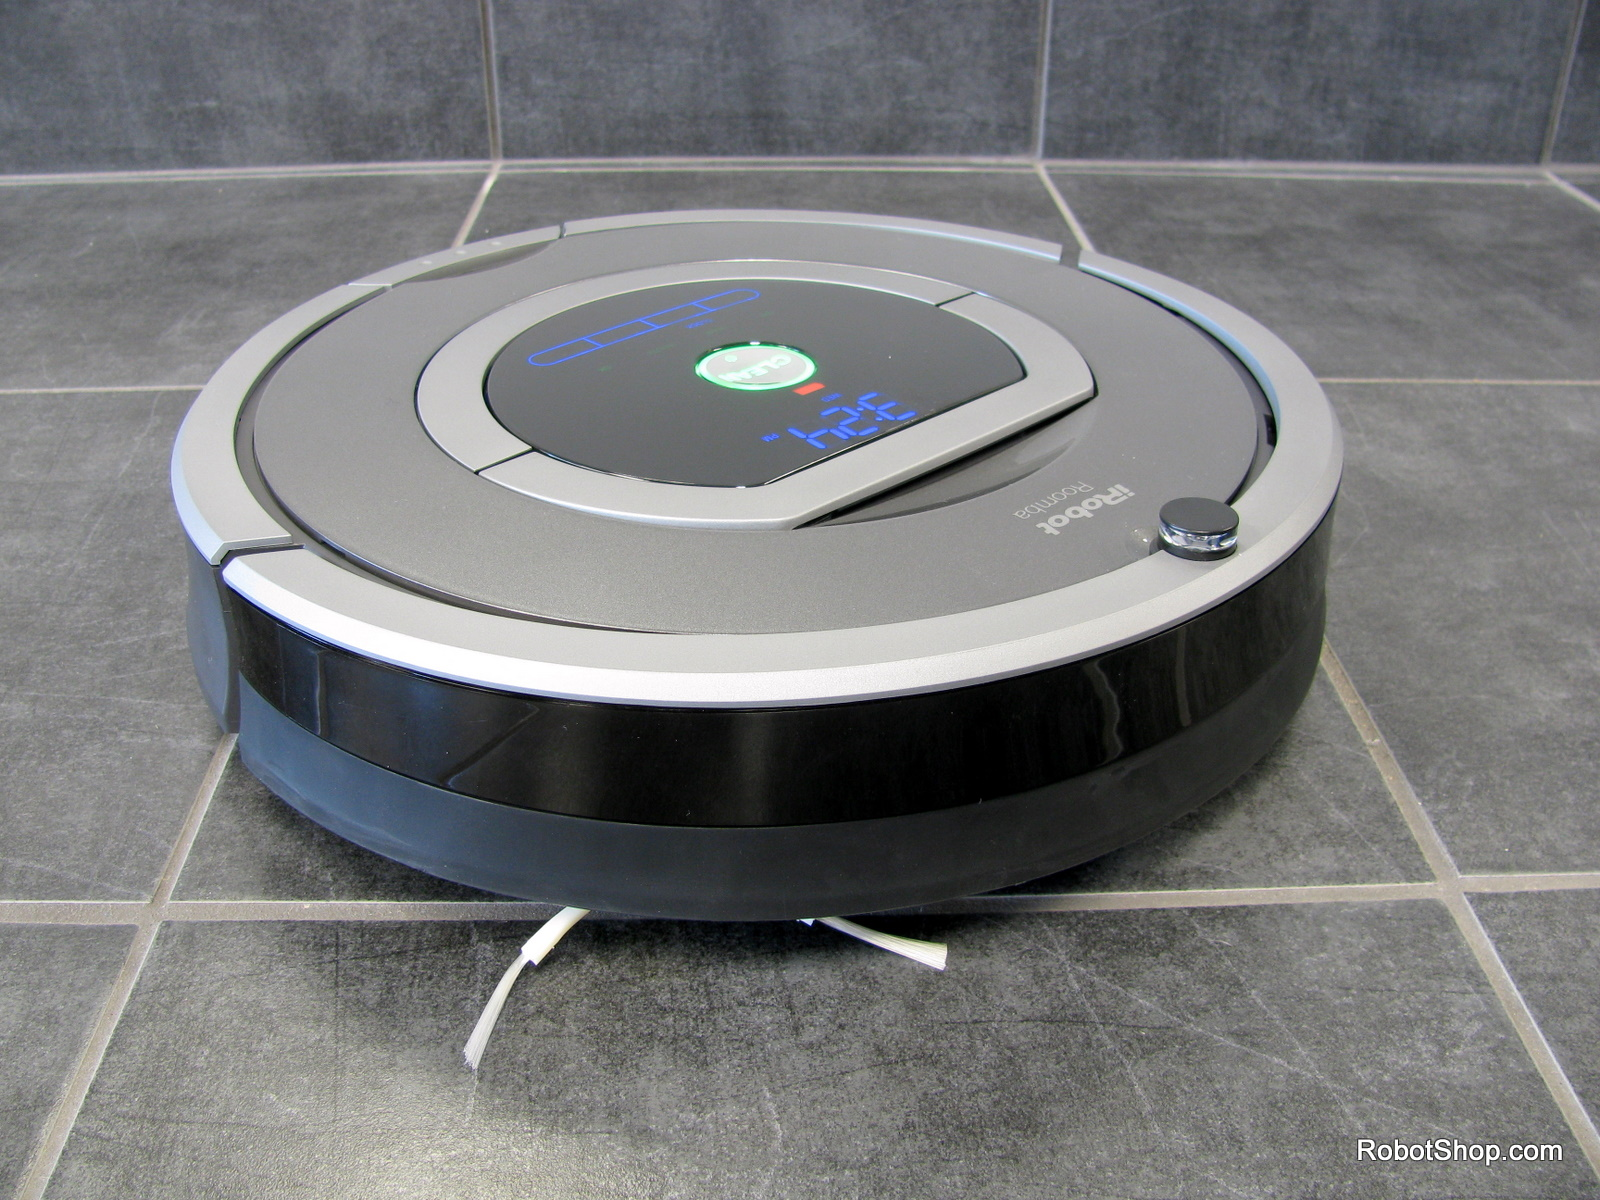
\includegraphics[width=67mm, keepaspectratio]{figures/iRobot_roomba_780.jpg}\hspace{1cm}
	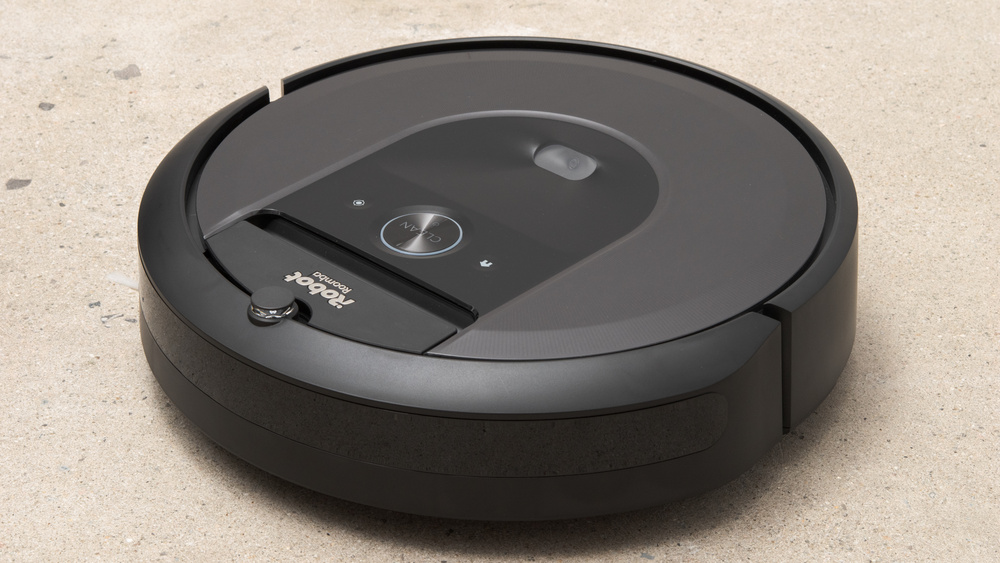
\includegraphics[width=67mm, keepaspectratio]{figures/iRobot_roomba_i7.jpg}\\\vspace{5mm}
	\caption{iRobot Roomba 780 (left) and i7 (right) (sources: \cite{roomba780}\cite{roombai7})}
	\label{fig:Roombas}
\end{figure}
\FloatBarrier
This example highlights the advantages of simultaneous localization and mapping (SLAM) in a household environment. SLAM technology is also transformative in industrial contexts. For instance, autonomous robots can transport heavy products across large warehouses. In such scenarios, a wall-to-wall navigation algorithm would be impractical, as it would likely fail to reach its destination before depleting its battery. Consequently, modern autonomous systems increasingly rely on SLAM algorithms to enable efficient and reliable navigation.

In summary, SLAM plays an essential role in empowering mobile robots to understand and navigate their environments effectively, whether in homes or complex industrial settings.


\section{Goal of the Thesis}

The primary objective of this thesis is to advance the navigation and exploration capabilities of a mobile robot, enabling it to independently explore and map a new environment upon arrival. The resulting map can then be reused by the robot itself or shared with other robots, supporting coordinated navigation and interaction in shared spaces.

The main focus of this work is to implement Visual SLAM (V-SLAM) using a stereo camera, as opposed to traditional SLAM methods that rely on LIDAR. This choice offers several advantages:
\begin{itemize}
\setlength\itemsep{0em}
    \item Stereo cameras can capture detailed 3D maps or point clouds, enhancing the robot's spatial awareness.
    \item Images taken at keyframes can be extracted to create photorealistic models of the environment, providing an immersive, realistic visual record.
    \item The camera enables additional functionalities, such as object detection and recognition, which can enrich the robot's understanding and interaction with its surroundings.
\end{itemize}

In addition to these core objectives, two optional goals were pursued:
\begin{itemize}
\setlength\itemsep{0em}
    \item Person detection and tracking: Using the camera to identify and track people, allowing the robot to either follow or avoid them as needed.
    \item Photorealistic scene reconstruction: Generating high-quality, realistic representations of the environment to support advanced visualization and mapping.
\end{itemize}

Through these goals, this thesis aims to enhance the utility, versatility, and adaptability of mobile robots in various environments by leveraging advanced visual SLAM techniques.


\section{Structure of the thesis}

During the writing of my thesis, I have gained significant experience in many fields. First, I learned about mobile robots, OAK-D cameras, neural reconstruction and 3D mapping in Chapter~\ref{related_works}, then I digged deeper in the capabilities of the OAK-D camera in Chapter~\ref{experiments_oak_d}, experimented with NeRFs and Gaussian Splatting in Chapter~\ref{nerf_gsplat}. After these I gained experience in 3D mapping using RTAB-Map, nvblox and Isaac VSLAM in Chapter~\ref{experiments_3d_mapping}. Then, I started the implementation of the mapping and photorealistic reconstruction pipeline in Chapter~\ref{implementation}. After the implementation I evaluated what I created in Chapter~\ref{evaluation}. Last but not least we suggested some future plans for the project in Chapter~\ref{future_plans}.
